\documentclass{beamer}
\usepackage[utf8]{inputenc}
\usetheme{Madrid}
\usecolortheme{default}
\usepackage{amsmath,amssymb,amsfonts,amsthm}
\usepackage{txfonts}
\usepackage{tkz-euclide}
\usepackage{listings}
\usepackage{adjustbox}
\usepackage{array}
\usepackage{tabularx}
\usepackage{gvv}
\usepackage{lmodern}
\usepackage{circuitikz}
\usepackage{tikz}
\usepackage{graphicx}
\setbeamertemplate{page number in head/foot}[totalframenumber]
\definecolor{bg}{gray}{0.95}
\lstset{
    language=C,
    basicstyle=\ttfamily\small,
    keywordstyle=\color{blue},
    stringstyle=\color{orange},
    commentstyle=\color{green!60!black},
    numbers=left,
    numberstyle=\tiny\color{gray},
    breaklines=true,
    showstringspaces=false,
}

\title{4.13.10}
\author{Aditya Mishra - EE25BTECH11005}
\date{September 30, 2025}

\begin{document}

\begin{frame}
\titlepage
\end{frame}

\begin{frame}{Question}
Vertices of a triangle are:
\[
\vec{A} = \myvec{-1 \\ -7}, \quad
\vec{B} = \myvec{5 \\ 1}, \quad
\vec{C} = \myvec{1 \\ 10}.
\]
Find the equation of the bisector of \(\angle ABC\).
\end{frame}

\begin{frame}{Solution}
Define vectors:
\[
\vec{D} = \vec{A} - \vec{B} = \myvec{-6 \\ -8}, \quad
\vec{E} = \vec{C} - \vec{B} = \myvec{-4 \\ 9}.
\]

Magnitudes:
\[
\|\vec{D}\|=10, \quad \|\vec{E}\|=\sqrt{97}.
\]
\end{frame}

\begin{frame}{Solution}
Normalized vectors:
\[
\vec{e}_D = \frac{1}{10} \myvec{-6 \\ -8}, \quad
\vec{e}_E = \frac{1}{\sqrt{97}} \myvec{-4 \\ 9}.
\]

Angle bisector vector:
\[
\vec{L} = \vec{e}_D + \vec{e}_E = \myvec{-\frac{6}{10} - \frac{4}{\sqrt{97}} \\
-\frac{8}{10} + \frac{9}{\sqrt{97}}}.
\]
\end{frame}

\begin{frame}{Solution}
Line along bisector passing through \(\vec{B}\):
\[
\vec{x} = \vec{B} + \lambda \vec{L}, \quad \lambda \in \mathbb{R}.
\]

Expanded:
\[
\vec{x} = \myvec{5 \\ 1} + \lambda \myvec{-\frac{6}{10} - \frac{4}{\sqrt{97}} \\ -\frac{8}{10} + \frac{9}{\sqrt{97}}}.
\]
\end{frame}
\begin{frame}{Plot}
\begin{figure}
    \centering
    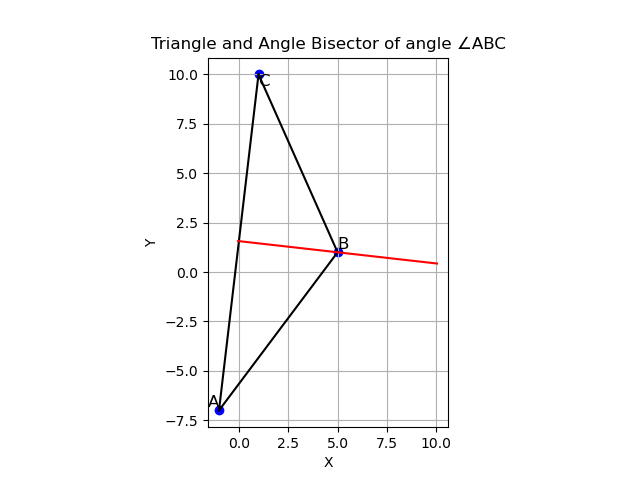
\includegraphics[width=0.8\columnwidth]{Figs/Figure_1.png}
\end{figure}
\end{frame}

\begin{frame}{Codes}
\centering
For Codes, refer to the URL below:  
\url{https://github.com/Aditya-Mishra11005/ee1030-2025/tree/temp/ee25btech11005/matgeo/4.13.10/Codes}
\end{frame}
\end{document}

